\section{Introduction}

In high-dimensional settings, the information captured by the relatively few
labeled training samples is not sufficient for training estimators with good
predictive performance. Therefore, to select among the set of feasible
solutions, one needs to assume a certain structural bias for the estimator
% However, the learning problem becomes tractable if the ground truth has
% certain structural properties that are known a priori
(e.g.\ sparsity, invariance to rotations, translations etc).
For deep neural networks (DNNs), this inductive bias is implicit and recent work [TODO
cite chizat] has revealed that it favors ``sparse'' solutions, similar to an
$\ell_1$ penalty. Moreover, work by \citet{soudry18,Ji20} has shown that
minimizing an exponential loss (e.g.\ logistic, softmax) on separable data leads
to the solution that maximizes the minimum margin on the training set (we refer
to this as the \emph{min-margin solution}).

In order to better understand the behavior of overparameterized neural networks,
in this paper we study simple linear predictors that mirror the structure that
has been observed for DNNs. In particular, we focus on binary classification
with a linear and sparse ground truth. We study the interpolator that maximizes
the min-$\ell_1$-margin (i.e.\ basis pursuit), since a small $\ell_1$ norm is
known to induce sparsity \citep{tibshirani96}.

\begin{figure}[t]
  \centering
  
\includegraphics[width=\columnwidth]{figures/teaser_sketch.png}

%   \begin{subfigure}[t]{\textwidth}
%     \centering
%     \includegraphics[width=\textwidth]{figures/teaser_p_al_worse.pdf}
%   \end{subfigure}

  \caption{Two-dimensional sketch of the average-margin ($\am$) and min-margin
  classifiers ($\mm$). Unlike $\mm$, the average-margin interpolator depends on
\emph{all} the training points. Therefore, it is more stable given different
draws of the data (top vs bottom row). This phenomenon is even more pronounced
in high dimensions.}
\label{fig:teaser}

\end{figure}

Despite a large trove of positive results for maximum min-margin interpolation
in high dimensions \citep{Hastie22, wang22}, a recent work \citep{konstantin}
finds that predictors obtained with basis pursuit tend to exhibit larger
variance in high dimensions. Despite using the right structural bias, maximizing
the min-$\ell_1$-margin can even lead to larger error than its $\ell_2$
counterpart solely due to this increase in variance. This observation raises the
following natural question:

\begin{center}

\emph{Can we achieve lower variance while still exploiting the sparsity-inducing
bias of $\ell_1$ interpolation?}

\end{center}

\begin{figure*}[t]
  \centering
  \begin{subfigure}[t]{0.24\linewidth}
    \centering
    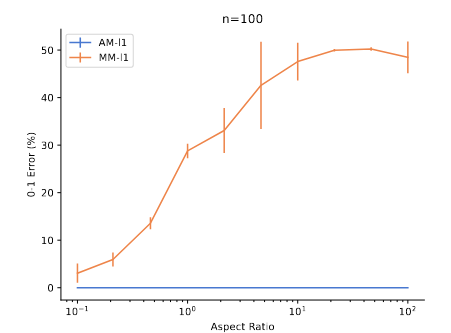
\includegraphics[width=\columnwidth]{figures/estim_err_s1.png}
    \label{fig:estim_err_s1}
    \caption{}
  \end{subfigure}
  \hfill
  \begin{subfigure}[t]{0.24\linewidth}
    \centering
    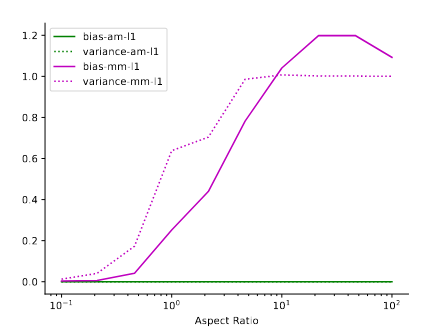
\includegraphics[width=\columnwidth]{figures/bias_variance_s1.png}
    \label{fig:bias_variance_s1}
    \caption{}
  \end{subfigure}
  \hfill
  \begin{subfigure}[t]{0.24\linewidth}
    \centering
    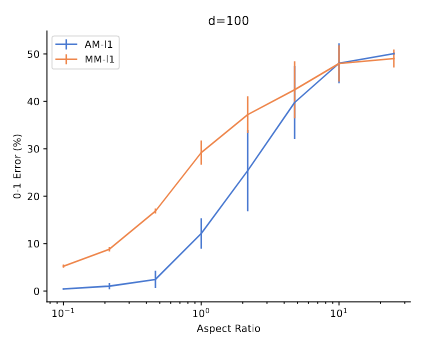
\includegraphics[width=\columnwidth]{figures/estim_err_s5.png}
    \label{fig:estim_err_s5}
    \caption{}
  \end{subfigure}
  \hfill
  \begin{subfigure}[t]{0.24\linewidth}
    \centering
    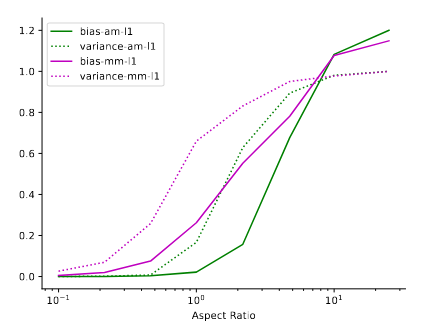
\includegraphics[width=\columnwidth]{figures/bias_variance_s5.png}
    \label{fig:bias_variance_s5}
    \caption{}
  \end{subfigure}

  \caption{The average-margin solution has lower estimation error than the
    min-margin interpolator in high dimensions (a, c). This is due to both a
    decrease in variance, but also a reduced bias (b, d). We use the
    distribution described in Section~\ref{sec:setting}, with a $1$-sparse (a,
    b) and a $5$-sparse (c, d) ground truth. For all experiments we set
  $d=???$\at{TODO}.}
  \label{fig:gmm_experiments}

\end{figure*}



In this paper, we propose to reduce the variance by minimizing the
\emph{average}-$\ell_1$-margin instead of the \emph{min}-$\ell_1$-margin.
Intuitively, in high-dimensions, the average-margin solution is determined by
all training points, unlike the min-margin interpolator. This intuition is
depicted in the sketch in Figure~\ref{fig:teaser}. Our results indicate that, in
high dimensions, average-margin interpolation does indeed lead to lower
variance, and hence, lower estimation error. Surprisingly, we our experiments
reveal that the average-margin solution also has lower bias, compared to the
min-margin interpolator.  Finally, in Section~\ref{sec:limitations} we argue
that despite its benefits in high-dimensions, the average-$\ell_1$-margin
estimator cannot readily replace min-margin interpolation in all settings. In
particular, we show that the average-margin solution is less robust to outliers
in low dimensions.





